\documentclass{article}

\setlength{\headsep}{0.75 in}
\setlength{\parindent}{.3 in}
\setlength{\parskip}{0.1 in}


%=====================================================
% Add PACKAGES Here (You typically would not need to):
%=====================================================

\usepackage{xcolor}
\usepackage[margin=1in]{geometry}
\usepackage{amsmath,amsthm}
\usepackage{fancyhdr}
\usepackage{enumitem}
\usepackage{graphicx}
\usepackage[export]{adjustbox}

%=====================================================
% Ignore This Part (But Do NOT Delete It:)
%=====================================================

\theoremstyle{definition}
\newtheorem{problem}{Problem}
\newtheorem*{fun}{Fun with Algorithms}
\newtheorem*{challenge}{Challenge Yourself}
\def\fline{\rule{0.75\linewidth}{0.5pt}}
\newcommand{\finishline}{\begin{center}\fline\end{center}}
\newtheorem*{solution*}{Solution}
\newenvironment{solution}{\begin{solution*}}{{\finishline} \end{solution*}}
\newcommand{\grade}[1]{\hfill{\textbf{($\mathbf{#1}$ points)}}}
\newcommand{\thisdate}{\today}
\newcommand{\thissemester}{\textbf{Rutgers: Spring 2021}}
\newcommand{\thiscourse}{CS 440: Artificial Intelligence} 
\newcommand{\thishomework}{Number} 
\newcommand{\thisname}{Name} 
\newcommand{\thisextension}{Yes/No} 


\headheight 40pt              
\headsep 10pt
\renewcommand{\headrulewidth}{0pt}
\lhead{\small \textbf{ Rutgers University.}}
\pagestyle{fancy}


\newcommand{\thisheading}{
   \noindent
   \begin{center}

   \framebox{
      \vbox{\vspace{2mm}
    \hbox to 6.28in { \textbf{\thiscourse \hfill \thissemester} }
       \vspace{4mm}
       \hbox to 6.28in { {\Large \hfill Artificial Inteligence \hfill} }
       \vspace{2mm}
         \hbox to 6.28in { { \hfill Homework: Search And Destroy  \hfill} }
       \vspace{2mm}
       \hbox to 6.28in { \emph{By: \thisname \hfill NetId: \thisextension}}
      \vspace{2mm}}
      }
   \end{center}
   \bigskip
}

%=====================================================
% Some useful MACROS (you can define your own in the same exact way also)
%=====================================================


\newcommand{\ceil}[1]{{\left\lceil{#1}\right\rceil}}
\newcommand{\floor}[1]{{\left\lfloor{#1}\right\rfloor}}
\newcommand{\prob}[1]{\Pr\paren{#1}}
\newcommand{\expect}[1]{\Exp\bracket{#1}}
\newcommand{\var}[1]{\textnormal{Var}\bracket{#1}}
\newcommand{\set}[1]{\ensuremath{\left\{ #1 \right\}}}
\newcommand{\poly}{\mbox{\rm poly}}


%=====================================================
% Fill Out This Part With Your Own Information:
%=====================================================


\renewcommand{\thishomework}{0} %Homework number
\renewcommand{\thisname}{Wilson Peralta, Krit Bhattarai} % Enter your name here
\renewcommand{\thisextension}{wrp29, kkb62} % Pick only one of the two options accordingly


\begin{document}


\thisheading

\indent\indent\indent\indent\indent\indent\indent\indent\indent\indent\textbf{Abstract}\\

\noindent This tesis explores the idea of modeling knowledge/belief about a system probabilistically, and use this beliefstate to efficiently direct future action. 

\noindent\textbf{Data Representation}\\
%  \hbox to 6.28in { {\Large \hfill Artificial Inteligence \hfill} }
   %    \vspace{2mm}
We represented the environment as a matrix of size dim*dim. Enumerating from 0-3 the terrain types (‘flat’,‘hilly’, ‘forested’, ‘caves and tunnels’) respectively. \\ As well as representing how difficult they are to search with probabilities 0.9, 0.7, 0.3, and 0.1 respectively.\\

\noindent Information on current time T is (the observations t AND failure to find target in searched cell J)\\
Updating our belief is based on if the environment does contain the target, the search will return failure or success with the appropriate probabilities, based on the terrain type.  If the search returns failure, for whatever reason, use this observation about the selected cell to update our belief state for all known cells. At the start all cells have equal probability, so the agent will choose one at random. Then the criteria to update agent is based on:\\
\indent\indent -To minimize false negatives, we ensure we search on a given cell as many times as the probability of failing, i.e in caves we have a probability of success in finding the target of 0.1. Therefore, we search in a given cell at least 10 times to ensure our probability is increased to 1. Meaning if the target was in a given location it must have found it, and it updates information accordingly. \\
Example, if we have a 5x5 environment initial probability is 1/25, after agent searches a cell:\\
\indent\indent -Target was found, and it terminates.\\
\indent\indent -Target was not found, we search T times according to probability of false negative and then update our belief using Bayes’ theorem. 
Original probability was 1, now after first search 1 * 1/250 + 24 * 1/25 = 240/250, and so forth. \\
Process is repeated and information updated until the target is found. \\
Basic Agent 1:  Iteratively travel to the cell with the highest probability of containing the target, search that cell.  Repeat until the target is found.\\
\begin{figure}[h!]	
		\IfFileExists{agent1.pdf}{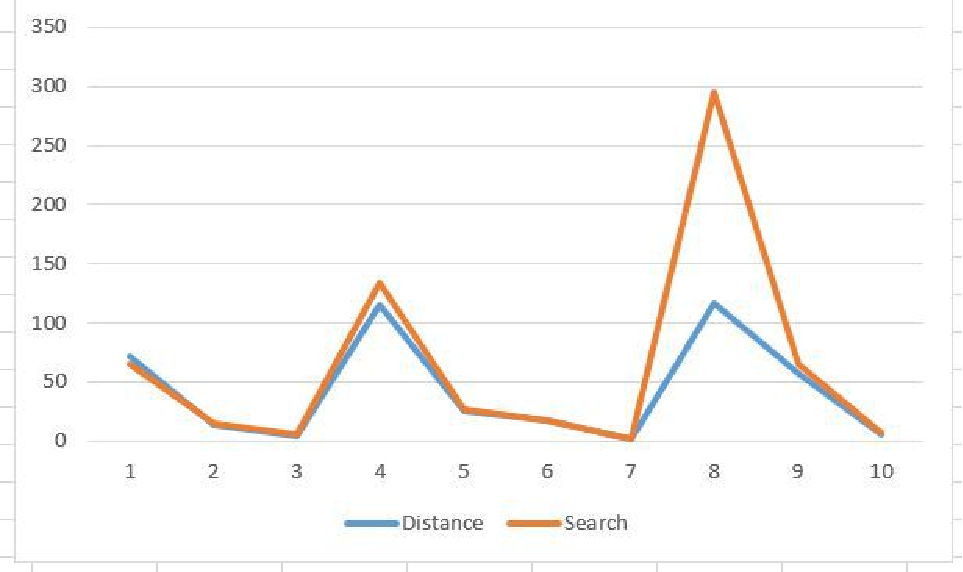
\includegraphics[width=0.6\textwidth,center]{agent1.pdf}}{No Figure Yet}
		\caption{ (Agent-1)} 
\end{figure}\\	

Basic Agent 2:  Iteratively travel to the cell with the highest probability of finding the target within that cell, search that cell.  Repeat until the target is found.\\
\noindent
\begin{figure}[h!]	
		\IfFileExists{agent2.pdf}{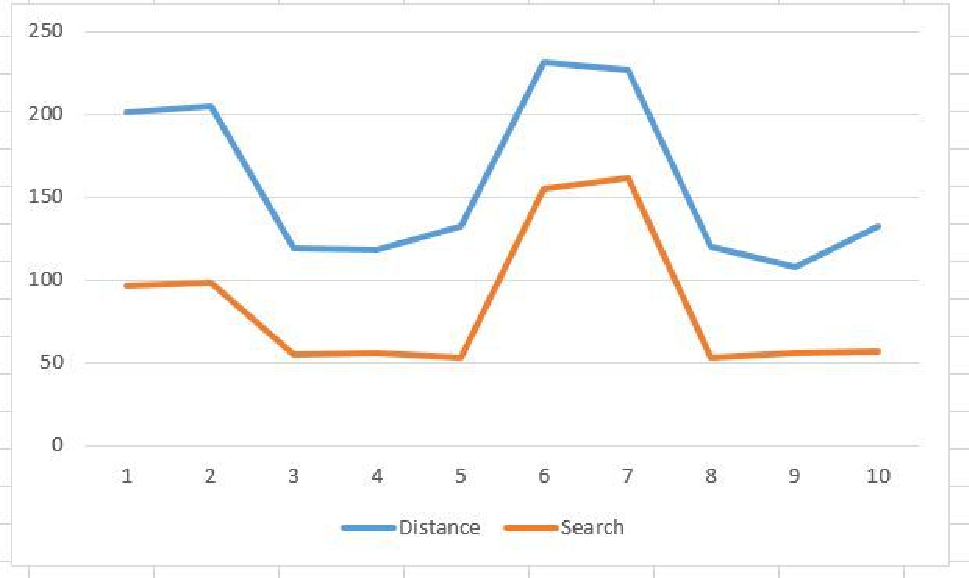
\includegraphics[width=0.6\textwidth,center]{agent2.pdf}}{No Figure Yet}
		\caption{ (Agent-2)} 
\end{figure}\\	
By graphs below we can clearly see that agent 1 is far more efficient than agent 2. Due to a fact as clear as water; although the chances of finding the chances are higher on some cells, the probability of the target being on those locations is closer to none. Therefore, searching the cells with higher probabilty of target being in said location, increments greatly the chances of finding the target faster.  	


\finishline

\end{document}